% Created 2018-03-03 Sat 01:07
\documentclass[a4j]{jsarticle}
\usepackage{orgstyle}
\rhead{Scalaで言語処理}

\providecommand{\alert}[1]{\textbf{#1}}

\title{Scalaで言語処理}
\author{田村直之}
\date{2018-03-03}
\hypersetup{
  pdfkeywords={},
  pdfsubject={},
  pdfcreator={Emacs Org-mode version 7.8.02}}

\begin{document}

\maketitle

\setcounter{tocdepth}{3}
\tableofcontents
\vspace*{1cm}
\thispagestyle{plain}
\vskip -10mm
\begin{comment}
\begin{itemize}
\item \href{file:///home/tamura/lect2/ProLang/2018/org/scala.org}{Top}
\item \href{file:///home/tamura/lect2/ProLang/2018/org/scala-list.org}{Scalaでリスト処理}
\item \href{file:///home/tamura/lect2/ProLang/2018/org/scala-recursive.org}{Scalaで再帰プログラミング}
\item \href{http://bach.istc.kobe-u.ac.jp/lect/tfpl/}{言語工学のページに戻る}
\item \href{file:///home/tamura/lect2/ProLang/2018/index.org}{プログラミング言語論のページに戻る}
\end{itemize}



\begin{itemize}
\item \href{file:///home/tamura/lect2/ProLang/2018/org/scala-complex.org}{Scalaで複素数計算}
\item \href{file:///home/tamura/lect2/ProLang/2018/org/scala-primeruler.org}{Scalaで素数ものさしを探す}
\item \href{file:///home/tamura/lect2/ProLang/2018/org/scala-sieve.org}{Scalaでエラトステネスの篩}
\item \href{file:///home/tamura/lect2/ProLang/2018/org/scala-parser.org}{Scalaで言語処理}
\end{itemize}



\end{comment}
\section{概要}
\label{sec-1}

\begin{quote}
Scalaのparser combinatorの機能を学び,電卓を作成する.
\end{quote}

以下は,作成中である.
\subsection{注意}
\label{sec-1-1}

\begin{comment}
  本Webページの作成には \href{http://orgmode.org/}{Emacs org-mode} を用い,
  数式等の表示は \href{http://www.mathjax.org}{MathJax} を用いています.
  IEでは正しく表示されないことがあるため,
  Firefox, Safari等のWebブラウザでJavaScriptを有効にしてお使いください.
  また \href{http://orgmode.org/worg/code/org-info-js/}{org-info.js} を利用しており,
  「m」キーをタイプするとinfoモードでの表示になります.
  利用できるショートカットは「?」で表示されます.
\end{comment}
\section{正規表現}
\label{sec-2}

Scalaプログラムでの正規表現 (regular expressions)は,与えられた文字列が正規表現で指定した
パターンにマッチするかどうかを調べるために用いられる.
なお,正規表現は,形式言語理論の正規言語 (regular languages),
すなわち有限オートマトン (finite automata)に対応している.

\begin{itemize}
\item 参考リンク: \href{https://ja.wikipedia.org/wiki/%E6%AD%A3%E8%A6%8F%E8%A1%A8%E7%8F%BE}{Wikipedia: 正規表現}
\end{itemize}

例えば,正規表現 \texttt{w*} は文字 \texttt{w} を0回以上繰り返したパターンを表しており,
空文字列および \texttt{w}, \texttt{ww}, \texttt{www}, \texttt{wwww} などにマッチする.
Scalaでの実行例は以下のようになる.

\begin{verbatim}
scala> "www".matches("w*")
res: Boolean = true

scala> "vvv".matches("w*")
res: Boolean = false
\end{verbatim}

同様に,正規表現 \texttt{w+} は文字 \texttt{w} を1回以上繰り返したパターンを表す.

\begin{verbatim}
scala> "www".matches("w+")
res: Boolean = true

scala> "".matches("w+")
res: Boolean = false
\end{verbatim}

複数の文字列の可能性があるパターンは $(r_1|r_2|\cdots|r_n)$ のように表す.
例えば \texttt{(A|T|G|C)+} は, \texttt{A} または \texttt{T} または \texttt{G} または \texttt{C} の文字を1回以上繰り返したパターンである.

\begin{verbatim}
scala> "ATTACCA".matches("(A|T|G|C)+")
res: Boolean = true
\end{verbatim}

上の例は, \texttt{[ATGC]+} と表すこともできる.
$[c_1c_2\cdots c_n]$ は,いずれかの文字 $c_i$ と一致するパターンを表す.

\begin{verbatim}
scala> "ATTACCA".matches("[ATGC]+")
res: Boolean = true
\end{verbatim}

正規表現 $[c_1c_2\cdots c_n]$ で,
\texttt{[0123456789]} のように選択肢の文字の文字コードが連続している場合には,
\texttt{[0-9]} のように文字の範囲を用いて記述できる.
例えば \texttt{[0-9]} は10進表記の1桁とマッチし, \texttt{[0-9a-fA-F]} は16進表記の1桁とマッチする.

\begin{verbatim}
scala> "2018".matches("[0-9]+")
res: Boolean = true

scala> "7E2".matches("[0-9a-fA-F]+")
res: Boolean = true
\end{verbatim}

さらに \texttt{[0-9]} は \texttt{\textbackslash{}d} と記述できる.
ただし,バックスラッシュはScalaも文字列記法中でエスケープ文字にあたるため,
Scalaプログラム中では \texttt{"\textbackslash{}\textbackslash{}d"} のように,バックスラッシュを2つ書く必要がある.
あるいは,エスケープ文字を無効にした文字列表記を用いて \texttt{"""\textbackslash{}d"""} と記述する.

\begin{verbatim}
scala> "2018".matches("\\d+")
res: Boolean = true

scala> "2018".matches("""\d+""")
res: Boolean = true

scala> "7E2".matches("""[\da-fA-F]+""")
res: Boolean = true
\end{verbatim}

パターン $r?$ は $r$ または空とマッチする記法である.
例えば \texttt{-?} は,文字列 \texttt{-} または空文字列とマッチする.
したがって,負の数を含む整数の10進表記とマッチする正規表現として \texttt{-?\textbackslash{}d+} が利用できる.

\begin{verbatim}
scala> "-2018".matches("""-?\d+""")
res: Boolean = true
\end{verbatim}

正規表現には,他にも様々な表現方法があるが,とりあえず以上で説明を終える.
Scalaで利用できる正規表現の詳細は,以下のページなどを参考にされたい.

\begin{itemize}
\item \href{https://docs.oracle.com/javase/jp/8/docs/api/java/util/regex/Pattern.html}{Java 8の正規表現}
\end{itemize}
\subsection{練習問題}
\label{sec-2-1}

\begin{enumerate}
\item 正規表現「 \texttt{(A*|T*|G*|C*)} 」は,どのような文字列にマッチするか.
\begin{description}
\item[(解答例)] 空文字列, \texttt{A}, \texttt{T}, \texttt{G}, \texttt{C}, \texttt{AA}, \texttt{TT}, \texttt{GG}, \texttt{CC}, \texttt{AAA}, \texttt{TTT}, \texttt{GGG}, \texttt{CCC} など.
\end{description}
\item 正規表現「 \texttt{(A*|T*|G*|C*)+} 」は,どのような文字列にマッチするか.
\begin{description}
\item[(解答例)] 正規表現「 \texttt{(A|T|G|C)*} 」と同じ文字列にマッチする.
\end{description}
\item \texttt{A}, \texttt{T}, \texttt{G}, \texttt{C} の文字だけからなる空でない文字列で,長さが3の倍数のものとマッチする正規表現は何か.
\begin{description}
\item[(解答例)] 例えば「 \texttt{([ATGC][ATGC][ATGC])+} 」である.
       繰り返しを表す記法 $\{m\}$ を用いれば,「 \texttt{([ATGC]\{3\})+} 」と書ける.
\end{description}
\item 正規表現「 \texttt{\textbackslash{}d+} 」は \texttt{007} など,先頭に余分な \texttt{0} がある場合にもマッチしてしまう.
     これを避けるには,どのような正規表現を用いれば良いか.
\begin{description}
\item[(解答例)] 「 \texttt{[1-9]\textbackslash{}d*} 」で良さそうだが, \texttt{0} とマッチしない.

\begin{verbatim}
scala> "0".matches("""[1-9]\d*""")
res: Boolean = false
\end{verbatim}
\end{description}
\end{enumerate}
       したがって「 \texttt{(0|[1-9]\textbackslash{}d*)} 」などとすれば良い.

\begin{verbatim}
scala> "0".matches("""(0|[1-9]\d*)""")
res: Boolean = true
\end{verbatim}
\begin{enumerate}
\item 正規表現「 \texttt{-?\textbackslash{}d+} 」は,先頭に余分な \texttt{0} がある場合にもマッチするだけでなく,
     \texttt{-0} にもマッチしてしまう.
     これを避けるには,どのような正規表現を用いれば良いか.
\begin{description}
\item[(解答例)] 「 \texttt{(0|-?[1-9]\textbackslash{}d*)} 」などとすれば良い.
\end{description}
\end{enumerate}
\section{文脈自由文法とEBNF}
\label{sec-3}

電卓で用いる数式の構文 (syntax)などは,
形式文法 (formal grammar)の一種である文脈自由文法 (context free languages)を用いて定義することができる.
文脈自由文法による文法定義には,
バッカス・ナウア記法 (Backus-Naur Form; BNF)を拡張したEBNFが用いられることが多い.
EBNFは,対象言語 (object language)の文法を定義する言語であるから,
メタ言語 (metalanguage)と呼ばれることがある.

\begin{itemize}
\item 参考リンク: \href{https://ja.wikipedia.org/wiki/%E5%BD%A2%E5%BC%8F%E6%96%87%E6%B3%95}{Wikipedia: 形式文法}
\item 参考リンク: \href{https://ja.wikipedia.org/wiki/%E6%96%87%E8%84%88%E8%87%AA%E7%94%B1%E6%96%87%E6%B3%95}{Wikipedia: 文脈自由文法}
\item 参考リンク: \href{https://ja.wikipedia.org/wiki/%E3%83%90%E3%83%83%E3%82%AB%E3%82%B9%E3%83%BB%E3%83%8A%E3%82%A6%E3%82%A2%E8%A8%98%E6%B3%95}{Wikipedia: バッカス・ナウア記法}
\item 参考リンク: \href{https://ja.wikipedia.org/wiki/EBNF}{Wikipedia: EBNF}
\item 参考リンク: \href{https://ja.wikipedia.org/wiki/%E3%83%A1%E3%82%BF%E8%A8%80%E8%AA%9E}{Wikipedia: メタ言語}
\end{itemize}

EBNFの具体的な書き方には,様々な流儀があるが,ここでは以下のように書くことにする.

\begin{itemize}
\item \textbf{終端記号} (terminal symbols; 対象言語の文字列): 
    \texttt{"a"} のようにダブル・クォーテーションでくくって表す.
\item \textbf{非終端記号} (nonterminal symbols; EBNFの記号): 
    \emph{expression} のようにイタリック文字で表記し,構文カテゴリーを表す.
\item \textbf{構文規則} (syntax rules): 
    以下のような形式で表し,非終端記号で表される文字列集合を定義する.
    \begin{align*}
    \mbox{非終端記号} & ::= \mbox{定義}
    \end{align*}
\end{itemize}

また,定義中に以下のような記法を使用する.


\begin{center}
\begin{tabular}{ll}
\hline
 EBNFでの記法              &  説明                             \\
\hline
 $\alpha_1\ \alpha_2$      &  $\alpha_1$ と $\alpha_2$ の連結  \\
 $\alpha_1 \mid \alpha_2$  &  $\alpha_1$ または $\alpha_2$     \\
 $\{\ \alpha\ \}$          &  $\alpha$ の0回以上の繰り返し     \\
 $[\ \,\alpha\ \,]$        &  $\alpha$ または空                \\
 $(\ \alpha\ )$            &  $\alpha$ のグループ化            \\
\hline
\end{tabular}
\end{center}



例えば,以下は10進数字を表す構文カテゴリー \emph{digit} と,
10進表記の整数を表す構文カテゴリー \emph{integer} を定義している.
\begin{align*}
  \textit{digit} & ::=\ 
  \mbox{"0"}\ \mid\ \mbox{"1"}\ \mid\ \mbox{"2"}\ \mid\ \mbox{"3"}\ \mid\ \mbox{"4"}\ \mid\ 
  \mbox{"5"}\ \mid\ \mbox{"6"}\ \mid\ \mbox{"7"}\ \mid\ \mbox{"8"}\ \mid\ \mbox{"9"} \\
  \textit{integer} & ::=\ 
  [\ \mbox{"-"}\ ]\ \textit{digit}\ \{\ \textit{digit}\ \}
\end{align*}
\section{前置記法の電卓}
\label{sec-4}
\subsection{構文定義}
\label{sec-4-1}

まず,文法が簡単な前置記法 (prefix notation)の電卓を考える.
すなわち,加減乗除算を
\texttt{+(x,y)}, \texttt{-(x,y)}, \texttt{*(x,y)}, \texttt{/(x,y)}
のように記述する記法である.
この記法だと,例えば $3+1-4*2$ は \texttt{-(+(3,1),*(4,2))} と記述する.

この構文は,EBNFで以下のように定義できる.

\begin{align*}
  \textit{expr} & ::=\ 
  \textit{integer}\ \mid\ 
  \textit{func}\ \mbox{"("}\ \textit{expr}\ \mbox{","}\ \textit{expr}\ \mbox{")"} \\
  \textit{func} & ::=\ 
  \mbox{"+"}\ \mid\ \mbox{"-"}\ \mid\ \mbox{"*"}\ \mid\ \mbox{"/"}
  %
\end{align*}

Scalaのparser combinatorを用いると,EBNFと同様の記法で構文を定義し,
与えられた文字列の構文解析を実現できる.
ただ,すべての構文定義を実現できるわけではない.
Scalaのparser combinatorは,
トップダウン型の再帰下降構文解析 (recursive descent parsing)のため
左再帰 (left recursive)な構文規則は利用できない.
しかし,それと同等の記述が可能であり,実用上は問題ない.

\begin{itemize}
\item 参考リンク: \href{http://www.scala-lang.org/api/current/scala-parser-combinators/scala/util/parsing/combinator/Parsers.html}{scala.util.parsing.combinator.Parsers}
\item 参考リンク: \href{http://www.artima.com/pins1ed/}{Programming in Scala, First Edition}: 31. Combinator Parsing
\item 参考リンク: \href{https://en.wikipedia.org/wiki/Parser%255Fcombinator}{Wikipedia: Parser combinator}
\item 参考リンク: \href{https://ja.wikipedia.org/wiki/%E5%86%8D%E5%B8%B0%E4%B8%8B%E9%99%8D%E6%A7%8B%E6%96%87%E8%A7%A3%E6%9E%90}{Wikipedia: 再帰下降構文解析}
\item 参考リンク: \href{https://ja.wikipedia.org/wiki/%E5%B7%A6%E5%86%8D%E5%B8%B0}{Wikipedia: 左再帰}
\end{itemize}

EBNFで,具体的に構文を定義しようとすると,空白の取り扱いが面倒になる.
数の文字列の途中に空白文字は許したくないが,コンマやカッコの前後には空白文字を許したい.
これを,EBNFで正しく定義しようとすると,たとえば以下のようになり,無駄に複雑だ.
\begin{align*}
  \textit{expr} & ::=\ 
  \textit{spaces}\ (\ 
  \textit{integer}\ \mid\ 
  \textit{func}\ \mbox{"("}\ \textit{expr}\ \mbox{","}\ \textit{expr}\ \mbox{")"}\ 
  )\ \textit{spaces} \\
  \textit{func} & ::=\ 
  \textit{spaces}\ (\ 
  \mbox{"+"}\ \mid\ \mbox{"-"}\ \mid\ \mbox{"*"}\ \mid\ \mbox{"/"}\ 
  )\ \textit{spaces} \\
  \textit{spaces} & ::=\ 
  \{\ \mbox{" "}\ \}
\end{align*}

そこで,数や変数名など途中に空白文字を許さない構文単位を \textbf{トークン} (token)と呼び,
トークンとトークンの間には自動的に空白を許すことにすれば便利だ.

\href{http://www.scala-lang.org/api/current/scala-parser-combinators/scala/util/parsing/combinator/JavaTokenParsers.html}{scala.util.parsing.combinator.JavaTokenParsers} では,
以下の関数が事前に定義されており,トークンとして利用可能である.


\begin{center}
\begin{tabular}{lll}
\hline
 関数名                        &  トークンの種類      &  例                                                                 \\
\hline
 \texttt{ident}                &  変数名などの識別名  &  \texttt{x}, \texttt{x1}, \texttt{名前} など                        \\
 \texttt{wholeNumber}          &  整数                &  \texttt{12}, \texttt{-34} など                                     \\
 \texttt{decimalNumber}        &  符号なし小数        &  \texttt{12}, \texttt{12.3}, \texttt{.14} など                      \\
 \texttt{floatingPointNumber}  &  浮動小数点数        &  \texttt{3.14}, \texttt{6.02e23} など                               \\
 \texttt{stringLiteral}        &  文字列              &  \texttt{"abc"}, \texttt{"\textbackslash{}\textbackslash{}d"} など  \\
\hline
\end{tabular}
\end{center}



なお JavaTokenParsers は \href{http://www.scala-lang.org/api/current/scala-parser-combinators/scala/util/parsing/combinator/RegexParsers.html}{scala.util.parsing.combinator.RegexParsers} のサブクラスになっており,
正規表現を用いて新たなトークンを定義することもできる.

前置記法の電卓を JavaTokenParsers で定義したプログラムは,
以下のように書ける(\href{file:///home/tamura/lect2/ProLang/2018/org/prog/parser/CalcP0.scala}{CalcP0.scala}).


\begin{verbatim}
import scala.util.parsing.combinator._

object CalcP0 extends JavaTokenParsers {
  def expr: Parser[Any] = integer | func ~ "(" ~ expr ~ "," ~ expr ~ ")"
  def func = "+" | "-" | "*" | "/"
  def integer = wholeNumber
}
\end{verbatim}

関数exprが前置記法の式の \textbf{パーサ} (parser; 構文解析器)である.
そして,関数funcが演算子の部分をパースするパーサ,
関数integerが整数の部分をパースするパーサとなっている.

関数exprの定義部分を見ればわかるように,
「または」はEBNFと同様に \texttt{"|"} を用いているが,「連結」には \texttt{"\textasciitilde{}"} を用いている.
その他の記法は以下のように対応しており,
Scalaのparser combinatorで,EBNFの記法をほぼ自然に記述できることがわかる.


\begin{center}
\begin{tabular}{lll}
\hline
 Scalaでの記法                      &  EBNFでの記法              &  説明                             \\
\hline
 $\alpha_1$ \~{} $\alpha_2$         &  $\alpha_1\ \alpha_2$      &  $\alpha_1$ と $\alpha_2$ の連結  \\
 $\alpha_1 \mid \alpha_2$           &  $\alpha_1 \mid \alpha_2$  &  $\alpha_1$ または $\alpha_2$     \\
 \texttt{rep(} $\alpha$ \texttt{)}  &  $\{\ \alpha\ \}$          &  $\alpha$ の0回以上の繰り返し     \\
 \texttt{opt(} $\alpha$ \texttt{)}  &  $[\ \,\alpha\ \,]$        &  $\alpha$ または空                \\
 \texttt{(} $\alpha$ \texttt{)}     &  $(\ \alpha\ )$            &  $\alpha$ のグループ化            \\
\hline
\end{tabular}
\end{center}



このプログラムは以下のようにすればScala REPL内から実行できるようになる
(Scalaを実行する同じフォルダ中にCalcP0.scalaが保存しておくこと).

\begin{verbatim}
$ scala
scala> :load CalcP0.scala
\end{verbatim}

まず,CalcP0オブジェクト中で定義されている関数を直接実行できるようにimport命令を実行する.

\begin{verbatim}
scala> import CalcP0._
\end{verbatim}
なお,import命令の実行は,プログラムをloadするたびに行う必要がある点に注意すること.

parseAll関数を用いると,与えた文字列に対して \textbf{構文解析} (parsing)を実行することができる.
例えば,以下は \texttt{+(12,34)} を \emph{expr} として構文解析した結果である.

\begin{verbatim}
scala> parseAll(expr, "+(12,34)")
res: CalcP0.ParseResult[Any] = [1.9] parsed: (((((+~()~12)~,)~34)~))
\end{verbatim}

出力中の \texttt{[1.9]} は,文字列 \texttt{+(12,34)} の1文字目から9文字目の前 (つまり最終文字)まで
構文解析できたことを表し,
\texttt{(((((+\textasciitilde{}()\textasciitilde{}12)\textasciitilde{},)\textasciitilde{}34)\textasciitilde{}))} が構文解析の結果として得られた \textbf{構文木} (parse tree)を文字列表示したものである.

この表示は,非常にわかりにくいが,以下のような構造になっている (わかるだろうか?).
\begin{verbatim}
 ((((("+" ~ "(") ~ "12") ~ ",") ~ "34") ~ ")")
\end{verbatim}

これを構文木として図示すると以下のようになる(トークンは四角の箱で表されている).

\begin{center}

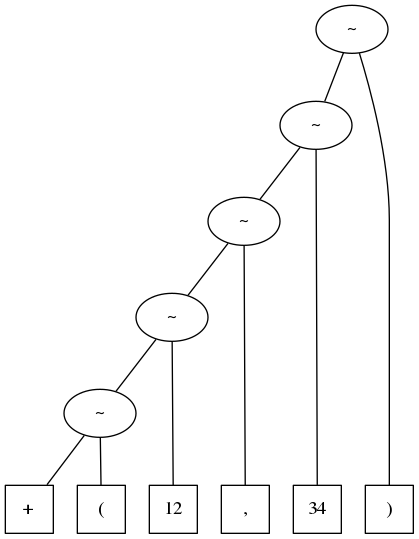
\includegraphics[width=0.3\textwidth]{images/scala-parse-tree1_aa424b059f845dce7ee0150628a229e0e65b7e0f.png}

\end{center}

\texttt{"+"}, \texttt{"("}, \texttt{"12"}, \texttt{","}, \texttt{"34"}, \texttt{")"} の各トークンに対し,
2項演算子 \texttt{"\textasciitilde{}"} で左結合的に対が作成されていることがわかる.

このように,得られた構文木中に意味的には不要なトークン(\texttt{"("}, \texttt{","}, \texttt{")"})が
含まれており,複雑になっている.

Scalaのparser combinatorには,不要な構造を削除する演算が用意されている.
演算子 \texttt{"\textasciitilde{}"} の代わりに  \texttt{"\textasciitilde{}>"} を用いると左側の構文解析結果が構文木から削除され,
\texttt{"<\textasciitilde{}"} を用いると右側の構文解析結果が構文木から削除される.

以下のプログラム \href{file:///home/tamura/lect2/ProLang/2018/org/prog/parser/CalcP1.scala}{CalcP1.scala} は, \texttt{"<\textasciitilde{}"} を用いて不要なトークンを結果の構文木から省いている.


\begin{verbatim}
import scala.util.parsing.combinator._

object CalcP1 extends JavaTokenParsers {
  def expr: Parser[Any] = integer | (func <~ "(") ~ (expr <~ ",") ~ (expr <~ ")")
  def func = "+" | "-" | "*" | "/"
  def integer = wholeNumber
}
\end{verbatim}

実行するには,以下のように入力する.

\begin{verbatim}
$ scala
scala> :load CalcP1.scala
scala> import CalcP1._
scala> parseAll(expr, "+(12,34)")
res: CalcP1.ParseResult[Any] = [1.9] parsed: ((+~12)~34)
\end{verbatim}

表示された結果は,以下のような構文木を表している.

\begin{center}

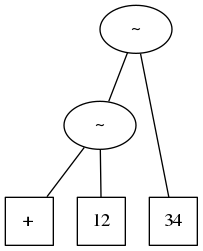
\includegraphics[width=0.15\textwidth]{images/scala-parse-tree2_606648ec1cbbbdeec1fc1887f438f8b6c2a3c21a.png}

\end{center}
\subsection{練習問題}
\label{sec-4-2}

\begin{enumerate}
\item CalcP1.scala を修正し,整数でなく浮動小数点数が利用できるようにせよ.
\begin{description}
\item[(解答例)] 例えば以下のように修正する(\href{file:///home/tamura/lect2/ProLang/2018/org/prog/parser/CalcP1float.scala}{CalcP1float.scala}).

\begin{verbatim}
def expr: Parser[Any] = number | (func <~ "(") ~ (expr <~ ",") ~ (expr <~ ")")
def func = "+" | "-" | "*" | "/"
def number = floatingPointNumber
\end{verbatim}
\end{description}
\end{enumerate}
\begin{enumerate}
\item CalcP1.scala を修正し \texttt{"-(12)"} や \texttt{"abs(-34)"} などの1引数の演算や関数を記述できるようにせよ.
\begin{description}
\item[(解答例)] 例えば以下のように修正する(\href{file:///home/tamura/lect2/ProLang/2018/org/prog/parser/CalcP1unary.scala}{CalcP1unary.scala}).

\begin{verbatim}
def expr: Parser[Any] =
  integer |
  (func1 <~ "(") ~ (expr <~ ")") |
  (func2 <~ "(") ~ (expr <~ ",") ~ (expr <~ ")")
def func1 = "-" | ident
def func2 = "+" | "-" | "*" | "/" | ident
def integer = wholeNumber
\end{verbatim}
\end{description}
\end{enumerate}
       ここでは,1引数の関数名として \texttt{ident} を許しているから,
       \texttt{abs} だけでなく任意の識別名が利用可能となっている.
       また,2引数の関数名としても任意の識別名が利用できるようにしている.
\begin{enumerate}
\item 以下の関数 \texttt{hexnum} を用いると \texttt{\#7E2} などの16進表記の整数をトークンとして利用できる.

\begin{verbatim}
def hexnum = "#" ~> "[0-9a-fA-F]+".r
\end{verbatim}
\end{enumerate}
     CalcP1.scala を修正し16進表記の整数を利用できるようにせよ.
\begin{description}
\item[(解答例)] 例えば \href{file:///home/tamura/lect2/ProLang/2018/org/prog/parser/CalcP1hex.scala}{CalcP1hex.scala} のように修正する.
\end{description}
\subsection{構文解析結果の利用}
\label{sec-4-3}

ここまでで,前置記法の式の構文解析が実現できた.
Scalaのparser combinatorでは,構文解析結果に対する処理を記述することもできる.
その機能を用いて,前置記法の電卓を実現しよう.
なお,ここでは計算結果は整数とし,浮動小数点の電卓の実現は練習問題とする.

\href{file:///home/tamura/lect2/ProLang/2018/org/prog/parser/CalcP1.scala}{CalcP1.scala} の expr の定義を見ると

\begin{verbatim}
def 関数名: Parser[Any] = 構文定義1 | 構文定義2 | ... | 構文定義n
\end{verbatim}
のようになっている.
これを,Scalaで整数を表すデータ型Intを返すようにするには,
以下のように記述する(わかりやすく改行を追加している).

\begin{verbatim}
def 関数名: Parser[Int] =
  構文定義1 ^^ Intを返す関数1 |
  構文定義2 ^^ Intを返す関数2 |
  ...
  構文定義n ^^ Intを返す関数n
\end{verbatim}
ここで「Intを返す関数i」は,「構文定義i」の構文解析結果を引数としてIntの結果を返す関数である.

expr の「構文定義1」は \texttt{integer} で,これは構文解析結果として文字列 (String)を返す.
したがって「Intを返す関数1」としては,10進整数の文字列表記からその値を求める関数を
記述すれば良い(データ型は \verb~String => Int~).

Scalaの匿名関数 (anonymous function)の機能を用いれば,
10進整数の文字列表記からその値を求める関数は \texttt{(s => s.toInt)} や
 \texttt{\{ s => s.toInt \}} と記述できる.
あるいは,さらに引数を省略して \texttt{(\_.toInt)} や \texttt{\{ \_.toInt \}} と記述しても良い.
すなわち,以下のような記述となる.

\begin{verbatim}
def expr: Parser[Int] =
  integer ^^ { _.toInt } |
  (func <~ "(") ~ (expr <~ ",") ~ (expr <~ ")") ^^ { t => ... }
\end{verbatim}

expr の「構文定義2」は \texttt{(func <\textasciitilde{} "(") \textasciitilde{} (expr <\textasciitilde{} ",") \textasciitilde{} (expr <\textasciitilde{} ")")} で,
\texttt{(("+" \textasciitilde{} 12) \textasciitilde{} 34)} などの構造が返ってきて,
そのデータ型は \texttt{\textasciitilde{}[\textasciitilde{}[String,Int],Int]} である.
データ構造 \texttt{(x \textasciitilde{} y)} の第一要素は \texttt{.\_1} のメソッドで,
第二要素は \texttt{.\_2} のメソッドで取り出すことができる.
つまり, \texttt{t} の値が \texttt{(("+" \textasciitilde{} 12) \textasciitilde{} 34)} の場合,
\texttt{t.\_1.\_2} で12を, \texttt{t.\_2} で34が得られる.

しかし,このように複雑な構造から必要なデータを取り出す場合,Scalaのmatch構文を用いることができる.

\begin{verbatim}
t match {
  case パターン1 => 処理1
  case パターン2 => 処理2
  ...
  case パターンn => 処理n
}
\end{verbatim}
この時,「パターン1」から順に \texttt{t} の構造とパターンマッチ (pattern matching)が行われ,
最初にマッチした「パターンi」に対して「処理i」が実行される.

expr の「構文定義2」は \texttt{(func <\textasciitilde{} "(") \textasciitilde{} (expr <\textasciitilde{} ",") \textasciitilde{} (expr <\textasciitilde{} ")")} に対するパターンは,
\texttt{f \textasciitilde{} x \textasciitilde{} y} のように書けるから,以下のような記述となる.

\begin{verbatim}
def expr: Parser[Int] =
  integer ^^ { _.toInt } |
  (func <~ "(") ~ (expr <~ ",") ~ (expr <~ ")") ^^ { t => t match {
    case f ~ x ~ y => ...
  }}
\end{verbatim}
構文定義中の \texttt{func} の部分が変数 \texttt{f} に, 
最初の \texttt{expr} の部分が変数 \texttt{x} に,
次の \texttt{expr} の部分が変数 \texttt{y} に代入される.
なお, \texttt{f} のデータ型は \texttt{String} , \texttt{x} と \texttt{y} のデータ型は \texttt{Int} である.

\texttt{f} に代入される値は \texttt{"+"}, \texttt{"-"}, \texttt{"*"}, \texttt{"/"} のいずれかだ.
したがって,パターンを以下のように4通り記述すれば,よりわかりやすくなる.

\begin{verbatim}
def expr: Parser[Int] =
  integer ^^ { _.toInt } |
  (func <~ "(") ~ (expr <~ ",") ~ (expr <~ ")") ^^ { t => t match {
    case "+" ~ x ~ y => ...
    case "-" ~ x ~ y => ...
    case "*" ~ x ~ y => ...
    case "/" ~ x ~ y => ...
  }}
\end{verbatim}

また \texttt{\{ t => t match \{ ... \} \}} は,単に \texttt{\{ ... \}} と省略して書くことができる.

\begin{verbatim}
def expr: Parser[Int] =
  integer ^^ { _.toInt } |
  (func <~ "(") ~ (expr <~ ",") ~ (expr <~ ")") ^^ {
    case "+" ~ x ~ y => ...
    case "-" ~ x ~ y => ...
    case "*" ~ x ~ y => ...
    case "/" ~ x ~ y => ...
  }
\end{verbatim}

加減乗除の各演算に対し,値を計算する処理を付け加えると以下のようになる
(\href{file:///home/tamura/lect2/ProLang/2018/org/prog/parser/CalcP2.scala}{CalcP2.scala}).


\begin{verbatim}
import scala.util.parsing.combinator._

object CalcP2 extends JavaTokenParsers {
  def expr: Parser[Int] =
    integer ^^ { _.toInt } |
    (func <~ "(") ~ (expr <~ ",") ~ (expr <~ ")") ^^ {
      case "+" ~ x ~ y => x + y
      case "-" ~ x ~ y => x - y
      case "*" ~ x ~ y => x * y
      case "/" ~ x ~ y => x / y
    }
  def func = "+" | "-" | "*" | "/"
  def integer = wholeNumber
}
\end{verbatim}

以下は,実行例である.

\begin{verbatim}
scala> :load CalcP2.scala
scala> import CalcP2._
scala> parseAll(expr, "+(*(1,2), *(3,4))")
res: CalcP2.ParseResult[Int] = [1.18] parsed: 14
\end{verbatim}
\subsection{練習問題}
\label{sec-4-4}

\begin{enumerate}
\item CalcP2.scala を修正し,整数でなく浮動小数点数が利用できるようにせよ.
     結果が \texttt{Double} となることに注意すること.
\begin{description}
\item[(解答例)] 例えば \href{file:///home/tamura/lect2/ProLang/2018/org/prog/parser/CalcP2float.scala}{CalcP2float.scala} のように修正する.
\end{description}
\item さらに修正し \texttt{"-(0.1)"}, \texttt{"abs(-2.3)"}, \texttt{"max(4, 5)"} などの演算および関数が利用できるようにせよ.
     なお,これらの関数は \texttt{math.abs(-2.3)}, \texttt{math.max((4, 5)} などとすれば計算できる.
     使用できる関数については \href{http://www.scala-lang.org/api/current/scala/math/}{scala.math} パッケージを参照のこと.
\begin{description}
\item[(解答例)] 例えば \href{file:///home/tamura/lect2/ProLang/2018/org/prog/parser/CalcP2float2.scala}{CalcP2float2.scala} のように修正する.
\end{description}
\end{enumerate}
\subsection{複数引数への拡張}
\label{sec-4-5}

さらに,
+(x$_1$, x$_2$, \ldots{}, x$_n$) のように,複数の引数を許すようにしよう (n $\ge$ 1).
この構文は,EBNFで以下のように定義できる.
\begin{align*}
  \textit{expr} & ::=\ 
  \textit{integer}\ \mid\ 
  \textit{func}\ \mbox{"("}\ \textit{expr}\ \{\ \mbox{","}\ \textit{expr}\ \}\ \mbox{")"}
\end{align*}
ここで $\{\ \alpha\ \}$ は $\alpha$ の0回以上の繰り返しを表している.

これは,Scalaのparser combinatorを用いれば以下のように記述できる
(\href{file:///home/tamura/lect2/ProLang/2018/org/prog/parser/CalcP3.scala}{CalcP3.scala}).


\begin{verbatim}
import scala.util.parsing.combinator._

object CalcP3 extends JavaTokenParsers {
  def expr: Parser[Any] =
    integer |
    (func <~ "(") ~ expr ~ (rep("," ~> expr) <~ ")")
  def func = "+" | "-" | "*" | "/" | ident
  def integer = wholeNumber
}
\end{verbatim}

\texttt{rep("," \textasciitilde{}> expr)} が $\{\ \mbox{","}\ \textit{expr}\ \}$ に対応している.
また,任意の識別子を関数名として利用できるよう, \texttt{func} の定義に \texttt{ident} を追加している.

このプログラムを \texttt{+(1,2,3,4)} に対して実行すると以下の結果になる.

\begin{verbatim}
scala> :load CalcP3.scala
scala> import CalcP3._
scala> parseAll(expr, "+(1,2,3,4)")
res: CalcP3.ParseResult[Any] = [1.11] parsed: ((+~1)~List(2, 3, 4))
\end{verbatim}

\texttt{rep("," \textasciitilde{}> expr)} の部分に対応する結果が整数のリスト \texttt{List(2,3,4)} となっていることがわかる.
したがって,整数の結果を計算するプログラムは以下のように書ける.

\begin{verbatim}
def expr: Parser[Int] =
  integer ^^ { _.toInt } |
  (func <~ "(") ~ expr ~ (rep("," ~> expr) <~ ")") ^^ {
    case "+" ~ x ~ ys => ...
    case "-" ~ x ~ ys => ...
    case "*" ~ x ~ ys => ...
    case "/" ~ x ~ ys => ...
  }
\end{verbatim}

\texttt{+(1,2,3,4)} の場合,変数 \texttt{x} に整数 \texttt{1} が代入され,
変数 \texttt{ys} に整数のリスト \texttt{List(2,3,4)} が代入される.
したがって,結果は \texttt{x + ys.sum} とすれば良い
(あるいは \texttt{(x +: ys).sum} でも良い).

\texttt{-(1,2,3,4)} の場合は $1-2-3-4$ を表すと考えれば,
同様に結果は \texttt{x - ys.sum} で良い.
また \texttt{*(1,2,3,4)} の場合は $1\times 2\times 3\times 4$ を表すと考えられるから,
結果は \texttt{x * ys.product} となり,
\texttt{/(1,2,3,4)} の場合も同様に \texttt{x / ys.product} で良いだろう.

しかし,引数の個数が1つの場合に問題が生じる.
\texttt{+(1)}, \texttt{-(1)}, \texttt{*(1)}, \texttt{/(1)} のいずれの場合も結果が \texttt{1} となる.
\texttt{+}, \texttt{*}, \texttt{/} についてはこの結果でも良いが,
\texttt{-(1)} の場合には \texttt{-1} を結果とすべきだろう.

これは,以下のようにプログラムすれば解決できる
(\href{file:///home/tamura/lect2/ProLang/2018/org/prog/parser/CalcP4.scala}{CalcP4.scala}).


\begin{verbatim}
import scala.util.parsing.combinator._

object CalcP4 extends JavaTokenParsers {
  def expr: Parser[Int] =
    integer ^^ { _.toInt } |
    (func <~ "(") ~ expr ~ (rep("," ~> expr) <~ ")") ^^ {
      case "+" ~ x ~ ys => x + ys.sum
      case "-" ~ x ~ Nil => - x
      case "-" ~ x ~ ys => x - ys.sum
      case "*" ~ x ~ ys => x * ys.product
      case "/" ~ x ~ ys => x / ys.product
    }
  def func = "+" | "-" | "*" | "/" | ident
  def integer = wholeNumber
}
\end{verbatim}

\texttt{ys} の箇所が空リスト \texttt{Nil} になる場合のcaseパターンを追加している.
\subsection{練習問題}
\label{sec-4-6}

\begin{enumerate}
\item CalcP4.scala で \texttt{parseAll(expr, "abs(-1)")} を実行するとどうなるか.
\begin{description}
\item[(解答例)] 構文解析は成功しているが,その後の値の計算で,
       対応するcaseパターンが存在しないため \texttt{scala.MatchError} が表示される.
\end{description}
\item CalcP4.scala を修正し \texttt{abs(x)} で \texttt{x} の絶対値を計算するように拡張せよ.
\begin{description}
\item[(解答例)] 以下の行を追加すれば良い.

\begin{verbatim}
case "abs" ~ x ~ Nil => math.abs(x)
\end{verbatim}
\end{description}
\end{enumerate}
\begin{enumerate}
\item CalcP4.scala を修正し,結果が \texttt{Int} でなく \texttt{BigInt} となるようにせよ.
     また \texttt{fact(x)} で \texttt{x} の階乗を計算するようにせよ.
     なお,10進表記の文字列 \texttt{s} について \texttt{BigInt(s)} とすれば,
     \texttt{BigInt} に変換できる.
\begin{description}
\item[(解答例)] 例えば \href{file:///home/tamura/lect2/ProLang/2018/org/prog/parser/CalcP4bigint.scala}{CalcP4bigint.scala} のように修正する.
\end{description}
\end{enumerate}
\section{課題1}
\label{sec-5}

以下からいくつかを選択し, \href{file:///home/tamura/lect2/ProLang/2018/org/prog/parser/Work1.scala}{Work1.scala} に対して拡張を行うこと.

\begin{enumerate}
\item xiすべての最大値を求める関数 \texttt{max(x1, x2, ..., xn)} を追加せよ.
\begin{description}
\item[(ヒント)] \texttt{BigInt} のリスト \texttt{ys} の最大値は \texttt{ys.max} で求めることができる.
\end{description}
\item 正の整数xとyの最大公約数を求める関数 \texttt{gcd(x, y)} を追加せよ.
   二つの \texttt{BigInt} の最小公倍数を求める方法については \href{http://www.scala-lang.org/api/current/scala/math/BigInt.html}{scala.math.BigInt} を参照.
\begin{description}
\item[(ヒント)] \texttt{BigInt} の \texttt{gcd} メソッドを使用する.
\end{description}
\item 正の整数xiすべての最大公約数を求める関数 \texttt{gcd(x1, x2, ... xn)} を追加せよ.
\begin{description}
\item[(ヒント)] \texttt{BigInt} のリストに対し \texttt{reduce} を用いると良い.
\end{description}
\item 正の整数xiすべての最小公倍数を求める関数 \texttt{lcm(x1, x2, ... xn)} を追加せよ.
\begin{description}
\item[(ヒント)] xとyの最小公倍数を求める関数 \texttt{lcm(x, y)} をScalaプログラム中で以下のように定義し,
     xiのリストに対して \texttt{reduce} を用いる.

\begin{verbatim}
def lcm(x: BigInt, y: BigInt) = ...
\end{verbatim}
\end{description}
\end{enumerate}
\begin{enumerate}
\item n番目のフィボナッチ数を求める関数 \texttt{fib(n)} を追加せよ.
\begin{description}
\item[(ヒント)] \href{file:///home/tamura/lect2/ProLang/2018/org/scala-recursive.org}{Scalaで再帰プログラミング} を参照し関数 \texttt{fib(n)} をoScalaプログラム中で定義する.
     なお \texttt{BigInt} の値 \texttt{x} を \texttt{Int} に変換するには \texttt{x.toInt} とする.
\end{description}
\item 西暦y年 (y $\ge$ 1900) m月d日のユリウス日 (JDN)を求める関数 \texttt{julius(y, m, d)} を追加せよ.
   今日のユリウス日から自分の誕生日のユリウス日を引けば,何日生きてきたかがわかる.
\begin{description}
\item[(ヒント)] ユリウス日 (JDN)の計算方法については \href{https://ja.wikipedia.org/wiki/ユリウス通日}{Wikipedia: ユリウス通日} 中の「グレゴリオ暦からの換算式」を参照.
     なお $(month - 3) \bmod 12$ の部分は \texttt{(month - 3) \% 12} として良い.
\end{description}
\item n番目の素数を求める関数 \texttt{prime(n)} を追加せよ.
   ただし素数の値は \texttt{Int} の範囲内として良い.なお,1番目の素数は2である.
\begin{description}
\item[(ヒント)] \href{file:///home/tamura/lect2/ProLang/2018/org/scala-primeruler.org}{Scalaで素数ものさしを探す} を参照.
\end{description}
\end{enumerate}
\subsection{テスト方法}
\label{sec-5-1}

テスト用のデータ \href{file:///home/tamura/lect2/ProLang/2018/org/prog/parser/test1.txt}{test1.txt} を同じフォルダにダウンロードし,
以下のように実行するとテストを実施できる.


\begin{verbatim}
scala> :load Work1.scala
scala> Work1.test
\end{verbatim}

\begin{itemize}
\item \texttt{OK} と表示された場合,構文解析に成功し,計算した結果が正しい.
\item \texttt{NG} と表示された場合,構文解析に成功したが,計算結果が正しくない.
\item \texttt{ERR} と表示された場合,構文解析でエラーが生じている.
\item \texttt{scala.MatchError} などと表示された場合は,プログラムの誤りである.
\end{itemize}
\section{日本語での数表記が可能な電卓への拡張}
\label{sec-6}

``二千十八'' など,日本語での数表記が可能な電卓へ拡張してみよう.

\href{file:///home/tamura/lect2/ProLang/2018/org/prog/parser/CalcP4.scala}{CalcP4.scala} の \texttt{expr} の定義を変更し,
日本語表記の文字列に対し整数を返す関数 \texttt{jint} を追加する.
また,整数を \texttt{Int} でなく \texttt{BigInt} で表すように変更する.


\begin{verbatim}
def expr: Parser[BigInt] =
  integer ^^ { BigInt(_) } |
  jint |
  (func <~ "(") ~ expr ~ (rep("," ~> expr) <~ ")") ^^ {
    case "+" ~ x ~ ys => x + ys.sum
    case "-" ~ x ~ Nil => - x
    case "-" ~ x ~ ys => x - ys.sum
    case "*" ~ x ~ ys => x * ys.product
    case "/" ~ x ~ ys => x / ys.product
  }
\end{verbatim}

まず ``一'' から ``九'' の一桁の表記を可能なプログラムを作成してみよう
(\href{file:///home/tamura/lect2/ProLang/2018/org/prog/parser/CalcPJ1.scala}{CalcPJ1.scala}).
プログラム中で \texttt{jint1} は一桁の数を構文解析し \texttt{BigInt} の値を返す関数である.


\begin{verbatim}
import scala.util.parsing.combinator._

object CalcPJ1 extends JavaTokenParsers {
  def expr: Parser[BigInt] =
    integer ^^ { BigInt(_) } |
    jint |
    (func <~ "(") ~ expr ~ (rep("," ~> expr) <~ ")") ^^ {
      case "+" ~ x ~ ys => x + ys.sum
      case "-" ~ x ~ Nil => - x
      case "-" ~ x ~ ys => x - ys.sum
      case "*" ~ x ~ ys => x * ys.product
      case "/" ~ x ~ ys => x / ys.product
    }
  def func = "+" | "-" | "*" | "/" | ident
  def integer = wholeNumber
  def jint = jint1
  def jint1 =
    "一" ^^ { _ => BigInt(1) } |
    "二" ^^ { _ => BigInt(2) } |
    "三" ^^ { _ => BigInt(3) } |
    "四" ^^ { _ => BigInt(4) } |
    "五" ^^ { _ => BigInt(5) } |
    "六" ^^ { _ => BigInt(6) } |
    "七" ^^ { _ => BigInt(7) } |
    "八" ^^ { _ => BigInt(8) } |
    "九" ^^ { _ => BigInt(9) }
}
\end{verbatim}

次に,これを ``二十三'' などの二桁の表記が可能なように拡張しよう.
二桁の数は ``二十'' や ``十三'' なども可能である.
つまり ``二十三'' での ``二'' や ``三'' の部分 (あるいは両方)が省略できる.
したがって,二桁以下の数を表す \texttt{jint2} の構文は以下のように定義できる.

\begin{verbatim}
def jint2 = opt(jint1) ~ "十" ~ opt(jint1) | jint1
\end{verbatim}

\texttt{opt(jint1)} は,空または \texttt{jint1} を表している.
\texttt{opt(jint1)} に対する構文解析結果のデータ型は \texttt{Option[BigInt]} となり,
空の場合は \texttt{None} という値を持ち,
空でない場合は \texttt{Some(x)} という値を持つ (\texttt{x} は \texttt{jint1} の結果).

したがって,二桁以下の表記が利用できるプログラム \href{file:///home/tamura/lect2/ProLang/2018/org/prog/parser/CalcPJ2.scala}{CalcPJ2.scala} は以下のようになる.


\begin{verbatim}
import scala.util.parsing.combinator._

object CalcPJ2 extends JavaTokenParsers {
  def expr: Parser[BigInt] =
    integer ^^ { BigInt(_) } |
    jint |
    (func <~ "(") ~ expr ~ (rep("," ~> expr) <~ ")") ^^ {
      case "+" ~ x ~ ys => x + ys.sum
      case "-" ~ x ~ Nil => - x
      case "-" ~ x ~ ys => x - ys.sum
      case "*" ~ x ~ ys => x * ys.product
      case "/" ~ x ~ ys => x / ys.product
    }
  def func = "+" | "-" | "*" | "/" | ident
  def integer = wholeNumber
  def jint = jint2
  def jint1 =
    "一" ^^ { _ => BigInt(1) } |
    "二" ^^ { _ => BigInt(2) } |
    "三" ^^ { _ => BigInt(3) } |
    "四" ^^ { _ => BigInt(4) } |
    "五" ^^ { _ => BigInt(5) } |
    "六" ^^ { _ => BigInt(6) } |
    "七" ^^ { _ => BigInt(7) } |
    "八" ^^ { _ => BigInt(8) } |
    "九" ^^ { _ => BigInt(9) }
  def jint2 =
    jint1 |
    (opt(jint1) <~ "十") ~ opt(jint1) ^^ {
      case None ~ None => BigInt(10)
      case Some(x1) ~ None => 10 * x1
      case None ~ Some(x2) => 10 + x2
      case Some(x1) ~ Some(x2) => 10 * x1 + x2
    }
}
\end{verbatim}

以下は,実行例である.

\begin{verbatim}
scala> :load CalcPJ2.scala
scala> import CalcPJ2._
scala> parseAll(expr, "+(一,二,三,四)")
res: CalcPJ2.ParseResult[BigInt] = [1.11] parsed: 10
\end{verbatim}

ただし, \texttt{jint2} の構文を以下のように定義すると ``二十'' の構文解析でエラーになってしまう.

\begin{verbatim}
def jint2 = jint1 | opt(jint1) ~ "十" ~ opt(jint1)
\end{verbatim}


\begin{verbatim}
scala> parseAll(expr, "二十")
res: CalcPJ2.ParseResult[BigInt] =
[1.2] failure: end of input expected

二十
 ^
\end{verbatim}

これは ``二十'' の構文解析で, \texttt{jint1} の規則の適用が ``二'' の部分に対して先に成功してしまい,
\texttt{opt(jint1) \textasciitilde{} "十" \textasciitilde{} opt(jint1)} の規則へ進まないためである.
したがって,文法定義の際には,このような点に注意しなければならない.

さらに,三桁の ``九百九十九'' 以下の値まで利用できる
プログラム \href{file:///home/tamura/lect2/ProLang/2018/org/prog/parser/CalcPJ3.scala}{CalcPJ3.scala} は以下のようになる.


\begin{verbatim}
import scala.util.parsing.combinator._

object CalcPJ3 extends JavaTokenParsers {
  def expr: Parser[BigInt] =
    integer ^^ { BigInt(_) } |
    jint |
    (func <~ "(") ~ expr ~ (rep("," ~> expr) <~ ")") ^^ {
      case "+" ~ x ~ ys => x + ys.sum
      case "-" ~ x ~ Nil => - x
      case "-" ~ x ~ ys => x - ys.sum
      case "*" ~ x ~ ys => x * ys.product
      case "/" ~ x ~ ys => x / ys.product
    }
  def func = "+" | "-" | "*" | "/" | ident
  def integer = wholeNumber
  def jint = jint3
  def jint1 =
    "一" ^^ { _ => BigInt(1) } |
    "二" ^^ { _ => BigInt(2) } |
    "三" ^^ { _ => BigInt(3) } |
    "四" ^^ { _ => BigInt(4) } |
    "五" ^^ { _ => BigInt(5) } |
    "六" ^^ { _ => BigInt(6) } |
    "七" ^^ { _ => BigInt(7) } |
    "八" ^^ { _ => BigInt(8) } |
    "九" ^^ { _ => BigInt(9) }
  def jint2 =
    (opt(jint1) <~ "十") ~ opt(jint1) ^^ {
      case None ~ None => BigInt(10)
      case Some(x1) ~ None => 10 * x1
      case None ~ Some(x2) => 10 + x2
      case Some(x1) ~ Some(x2) => 10 * x1 + x2
    } |
    jint1
  def jint3 =
    (opt(jint1) <~ "百") ~ opt(jint2) ^^ {
      case None ~ None => BigInt(100)
      case Some(x1) ~ None => 100 * x1
      case None ~ Some(x2) => 100 + x2
      case Some(x1) ~ Some(x2) => 100 * x1 + x2
    } |
    jint2
}
\end{verbatim}
\section{課題2}
\label{sec-7}

以下からいくつかを選択し, \href{file:///home/tamura/lect2/ProLang/2018/org/prog/parser/Work2.scala}{Work2.scala} に対して拡張を行うこと.

\begin{enumerate}
\item ``九千九百九十九'' 以下の値を利用できるようにせよ.
\begin{description}
\item[(ヒント)] 以下の構文定義を利用する.

\begin{verbatim}
def jint4 = (opt(jint1) <~ "千") ~ opt(jint3) | jint3
\end{verbatim}
\end{description}
\end{enumerate}
\begin{enumerate}
\item ``九千九百九十九万九千九百九十九'' 以下の値を利用できるようにせよ.
\begin{description}
\item[(ヒント)] 以下の構文定義を利用する.

\begin{verbatim}
def jintMan = (jint4 <~ "万") ~ opt(jint4) | jint4
\end{verbatim}
\end{description}
\end{enumerate}
\begin{enumerate}
\item ``九千九百九十九億九千九百九十九万九千九百九十九'' 以下の値を利用できるようにせよ.
\begin{description}
\item[(ヒント)] 以下の構文定義を利用する.

\begin{verbatim}
def jintOku = (jint4 <~ "億") ~ opt(jintMan) | jintMan
\end{verbatim}
\end{description}
\end{enumerate}
\begin{enumerate}
\item さらに ``兆'', ``京'', ``垓'' などを利用できるようにせよ (\href{https://ja.wikipedia.org/wiki/命数法}{Wikipedia: 命数法}).
\begin{description}
\item[(ヒント)] ``兆'' については以下の構文定義を利用する.

\begin{verbatim}
def jintCho = (jint4 <~ "兆") ~ opt(jintOku) | jintOku
\end{verbatim}
\end{description}
\end{enumerate}
\begin{enumerate}
\item ``きゅうひゃくきゅうじゅうきゅう'' など,ひらがなの表記を利用できるようにせよ.
\begin{description}
\item[(ヒント)] \texttt{jint1}, \texttt{jint2} などに規則を追加すれば良い.
\end{description}
\item \texttt{"和(1,2,3,4)} など,日本語で加減乗除を記述できるようにせよ.
   関数名は ``和'', ``差'', ``積'', ``商'' とすること.
\begin{description}
\item[(ヒント)] \texttt{expr} に規則を追加すれば良い.
\end{description}
\item \texttt{\#7E2} などの16進表記が可能になるようにせよ.
\begin{description}
\item[(ヒント)] 16進表記を許す構文規則については,以前の練習問題を参照.
     \texttt{BigInt("7E2", 16)} などとすれば,16進表記の文字列を \texttt{BigInt} に変換できる.
\end{description}
\item \texttt{"12k} で 12000, \texttt{"12M"} で 12000000 などを表せるようにせよ (\href{https://ja.wikipedia.org/wiki/SI%E6%8E%A5%E9%A0%AD%E8%BE%9E}{Wikipedia: SI接頭辞}).
\begin{description}
\item[(ヒント)] 以下の構文定義を利用する.

\begin{verbatim}
def expr: Parser[All] =
  integer ~ ("k" | "M" | "G" | "T" | "P") |
  integer |
  jint |
  (func <~ "(") ~ expr ~ (rep("," ~> expr) <~ ")")
\end{verbatim}
\end{description}
\end{enumerate}
\subsection{テスト方法}
\label{sec-7-1}

テスト用のデータ \href{file:///home/tamura/lect2/ProLang/2018/org/prog/parser/test2.txt}{test2.txt} を同じフォルダにダウンロードし,
以下のように実行するとテストを実施できる.


\begin{verbatim}
scala> :load Work2.scala
scala> Work2.test
\end{verbatim}

\begin{itemize}
\item \texttt{OK} と表示された場合,構文解析に成功し,計算した結果が正しい.
\item \texttt{NG} と表示された場合,構文解析に成功したが,計算結果が正しくない.
\item \texttt{ERR} と表示された場合,構文解析でエラーが生じている.
\item \texttt{scala.MatchError} などと表示された場合は,プログラムの誤りである.
\end{itemize}
\section{発展課題}
\label{sec-8}

\texttt{Work1.scala}, \texttt{Work2.scala} と同様に \texttt{Work3.scala} を作成し,自由に拡張を行え.
ただし,テスト用のデータ \texttt{test3.txt} を作成し \texttt{Work3.test} でテストを実行できるようにせよ.

以下は,拡張の例である.

\begin{enumerate}
\item 以下の構文規則を利用し, \texttt{3+1*4} などの挿入記法での通常の数式表記を可能にする.

\begin{verbatim}
def expr: Parser[Any] = opt("-") ~ term ~ rep("+" ~ term | "-" ~ term)
def term: Parser[Any] = factor ~ rep("*" ~ factor | "/" ~ factor)
def factor: Parser[Any] = integer | "(" ~> expr <~ ")" | (ident <~ "(") ~ expr ~ (rep("," ~> expr) <~ ")")
\end{verbatim}
\end{enumerate}
\begin{enumerate}
\item \texttt{"一足す二引く三"} など,日本語を用いた挿入記法での表記を可能にする.
\item \texttt{"MMXVIII"} など,ローマ数字の表記を可能にする (\href{https://ja.wikipedia.org/wiki/%E3%83%AD%E3%83%BC%E3%83%9E%E6%95%B0%E5%AD%97}{Wikipedia: ローマ数字}).
\item ``nine hundreds and ninety nine'' など,英語での表記を可能にする.
\item 複素数の計算を行う電卓を作成する.
\item 有理数 (分数)の計算を行う電卓を作成する.
\item ベクトルや行列の計算を行う電卓を作成する.
\end{enumerate}

\end{document}